% % !TeX program = xelatex
% !TeX spellcheck = es_ES
% !TeX encoding = utf8

\documentclass[onecolumn,10pt,titlepage,a4paper]{article}

\usepackage[a4paper,top=2.5cm,bottom=2cm,left=2cm,right=2cm,marginparwidth=1.75cm,headheight=28pt]{geometry}
% Formateo para castellano
%\usepackage[utf8]{inputenc}
\usepackage[spanish,mexico]{babel}
%\usepackage{natbib}


\newcommand{\celsius}{^\circ \mathrm{C}}
\newcommand{\air}{{\mathrm{humo}}}
%Bibliografía

% Simbolos para notas de pie
\usepackage[symbol]{footmisc}
\renewcommand*{\thefootnote}{\fnsymbol{footnote}}

% \renewcommand{\thefootnote}{\fnsymbol{footnote}}
% \footnote[num]{text}

% \pagestyle{myheading}
% \markright{Mi Documento \hfill Mi nombre \hfi}
%
\usepackage{fancyhdr,framed}
\setlength{\headheight}{15.2pt}
\pagestyle{fancy}
\lhead{Elementos Finitos II - 31.92 \\ Patricio Whittingslow -- 55423}
\chead{TP 2}


%\usepackage{subcaption}

% Para el entorno align


% Multiples columnas para glosario
\usepackage{multicol}

%Figuras y subtitulos
\usepackage{graphicx}
\usepackage{caption,subcaption}
\usepackage{hyperref}
\hypersetup{
    colorlinks,
    citecolor=black,
    filecolor=black,
    linkcolor=black,
    urlcolor=black
}
\usepackage[utopia,expert]{mathdesign} %Opcion "expert" para no romperme las smallcaps de helvetica. 
\usepackage{amsmath}

\newcommand{\rmfont}[1]{{\fontfamily{ptm}\selectfont%
		#1}}
\newcommand{\rmfontbf}[1]{{\fontfamily{ptm}\selectfont%
		\textbf{#1}}}
\newcommand{\rmfontsc}[1]{{\fontfamily{ptm}\selectfont%
		\textsc{#1}}}
    
\newcommand{\Matlab}{\rmfont{\sc Matlab}}
    \newcommand{\Adina}{{\sc ADINA}}
    \newcommand{\refp}[1]{(\ref{#1})}
    \newcommand{\unspace}{\!\!\!\!\!\!\!\!\!\!\!\!\!\!\!\!\!\!\!\!}
    \newcommand{\ms}{\ \ \ } %Matrix Spacing
    \newcommand{\di}{\textrm{d}}
    \newcommand{\jac}{\rmfontbf{J}}
    \newcommand{\Djac}{|\;\jac\;|}
    \newcommand{\dNi}{\di N_i}
    \newcommand{\sigmab}{\boldsymbol{\sigma}}
    \newcommand{\varepsilonb}{\boldsymbol{\varepsilon}}
    \newcommand{\Phib}{\boldsymbol{\Phi}}
    \newcommand{\CPhi}{\boldsymbol{\{ } \Phi \boldsymbol{\} }}
    \newcommand{\Mme}[1]{\boldsymbol{[}\mathbf{#1} \boldsymbol{]}}
    \newcommand{\Rme}[1]{\boldsymbol{\lfloor}\mathbf{#1} \boldsymbol{\rfloor}}
    \newcommand{\Cme}[1]{\boldsymbol{\{ }\mathbf{#1} \boldsymbol{\}} }
    \newcommand{\MB}{\Mme{B}}
    \newcommand{\MN}{\Mme{N}}
    \newcommand{\ME}{\Mme{E}}
    \newcommand{\Mk}{\Mme{k}}
    \newcommand{\MA}{\Mme{A}}
    \newcommand{\radial}{r}
    \newcommand{\eff}{f}
%Helvetica
\renewcommand{\familydefault}{\sfdefault}
\usepackage[scaled=1]{helvet}
\usepackage[format=plain,
            labelfont={bf,it},
            textfont=it]{caption}
%\usepackage[T1]{fontenc}
%--------------------------------------


\usepackage{siunitx}
\newcommand{\glossentry}[2]{$#1\ $ \indent #2 \par \vspace{.4cm} }
\newcommand{\adm}{\textrm{adm}}
\renewcommand\thepart{\Alph{part}}

\title{Informe Técnico - ITBA}

\author{Patricio Whittingslow}
%========================> Comienza Documento
\begin{document}
\begin{titlepage}
	\centering
	
	{ \large Instituto Tecnológico de Buenos Aires  \par }
	\vspace{2cm}
	{\Large \scshape Elementos Finitos II - 31.92 \par}
	\vspace{2cm}
	{\Huge \scshape Estudio de vibraciones de un motor utilizando el método de elementos finitos\par }
	\vspace{.5cm}
	{\Large  \par}
	\vspace{2cm}
	{\large \bf Autor \par}
	\vspace{.5cm}
	\textsc{\large Patricio Whittingslow -- 55423}
	\vspace{2cm}
	{\par \large Fecha de realización: \today \par}
	\vspace{1cm}
	{\large Fecha de entrega: .......................................\par}
	\vspace{\fill}
	{\large Firma del docente: .......................................}
	\vspace{\fill}
%	\begin{figure}[htb!]
%		\centering
%		
\includegraphics[width=6cm]{fig/logoitba.png}
%	\end{figure}
\end{titlepage}




\begin{multicols}{2}
	\section*{Glosario}
	\glossentry{\Cme{R}}{Vector de cargas externas.}
	\glossentry{\Mme{K}}{Matriz de rigidez.}
	\glossentry{\Mme{M}}{Matriz de masa.}
	\glossentry{\Cme{D}}{Vector de desplazamientos.}
	\glossentry{\chi}{Razón entre la frecuencia de excitación y la frecuencia natural del modo estudiado.}
	\glossentry{\Mme{C}}{Matriz de amortiguamiento.}
	\glossentry{L_c}{Longitud caracteristica de elemento. Parametro de refinado de malla.}
	\glossentry{\omega_e=\omega_{\mathrm{exc}}}{Frecuencia de excitacion [rad/s].}
\end{multicols}

\setcounter{section}{-1}

\tableofcontents

\section{Introducción Teórica}
Cuando se tiene una carga dependiente del tiempo la respuesta estructural también lo es. En el caso que sea un problema cuasiestático la resolución se puede hacer para los instantes de tiempos interesantes. Caso contrario se precisa efectuar un \textit{análisis dinámico}.
\begin{equation} \label{eq:FuerzasDinamicas}
	\text{Cuasiestático:}\quad \Mme{K}\Cme{D} = \Cme{R} \longrightarrow \text{Dinámico:} \quad 
	\Mme{M} \Cme{\ddot{D}} + \Mme{C}\Cme{\dot{D}} + \Mme{K}\Cme{D} = \Cme{R}
\end{equation}
	

donde el termino $\Mme{K}\Cme{D}$ suele ser referido como las \textit{fuerzas internas}, y $\Cme{R}$ siendo las \textit{fuerzas externas}.

El análisis dinámico busca la forma de deformación del sistema cuando este se encuentra excitado por cargas a una frecuencia cercana a la natural. La respuesta en deformación del sistema con una carga cíclica puede ser menor o mayor que con cargas estáticas de misma magnitud máxima, pero cuando la frecuencia de carga se acerca a la natural las deformaciones serán mucho mayor. 

Debido a este último punto es de sumo interés conocer la frecuencia natural de un sistema que tiene la posibilidad de someterse a una carga cíclica. Incluso puede ser de gran utilidad conocer el modo de deformación para entender como el sistema almacena energía.


\setcounter{section}{0}
\section{Problema}

\begin{itemize}
	\item Se precisa proponer un modelo para la estructura y representar gráficamente.
	\item Efectuar análisis modal y dimensionar las vigas del basamento. Considerar desplazamiento de $10$mm y $\omega_{\mathrm{exc}}=600\mathrm{rpm}$.
	\item Proponer un diseño alternativo superador teórico dejando de lado la perspectiva económica. Este diseño debe reducir cargas transmitidas y los desplazamientos del equipo.
\end{itemize}



\begin{figure}[htb!]
	\centering
	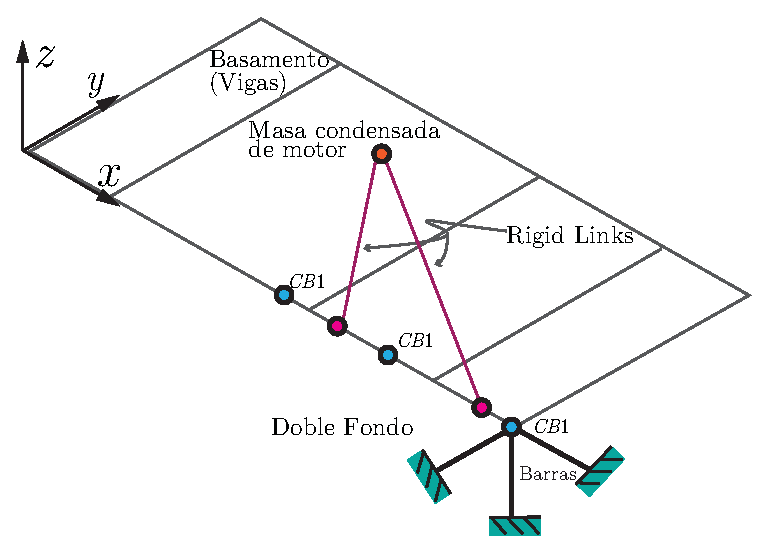
\includegraphics[width=0.6\textwidth]{fig/modelomotor.eps}
	\caption{Modelo del motor a grandes rasgos. El problema fue resuelto en \Matlab.}
	\label{fig:modelomotor}
\end{figure}

\section{Método}
El problema se resuelve en \Matlab{} utilizando el método de elementos finitos.

Elementos usados
\begin{itemize}
	\item Elemento masa 0D para masa puntual (sin rigidez) con momento de inercia
	\item Elementos viga Timoshenko con masa consistente para basamento
	\item Elementos viga para Rigid beams con rigidez de la vigas del basamento multiplicado por 2000 para modelar el motor como cuerpo rígido
	\item Elemento resorte para los bulones (nodos azules con $CB1$ en la figura \ref{fig:modelomotor}) con rigidez longitudinal de bulón $k_b$ en dirección $z$ y rigidez $\frac{k_b}{10}$ en $x$ e $y$ para representar el efecto de separar el motor del doble fondo con una resina.
\end{itemize}

Para el mallado se desarrollo un programa que cree los nodos y una los elementos automáticamente, tomando como input del usuario el tamaño nominal de los elementos viga. En la figura \ref{fig:modelobasamento} se ve el resultado de dicho programa con tamaño de elemento \textit{máximo.} Para la constante torsional $J_\tau$ se utilizó una formula aproximada para secciones rectangulares \eqref{eq:torsionalConstant}\footnote{Obtenido del libro \cite{young2002roark}}

\begin{equation} \label{eq:torsionalConstant}
J_{\tau}=h \cdot b^{3} \cdot\left(\frac{1}{3}-0,21 \cdot \frac{b}{h} \cdot\left(1-\frac{b^{4}}{12 \cdot h^{4}}\right)\right)
\end{equation}
donde $b$ es el lado corto y $h$ el lado largo.

Los bulones elegidos tienen 20mm de diámetro. Se usó este dato para calcular $k_b=\frac{E\pi d^2/4}{L}$.


\begin{figure}[htb!]
	\centering
	\begin{subfigure}{0.49\textwidth}
		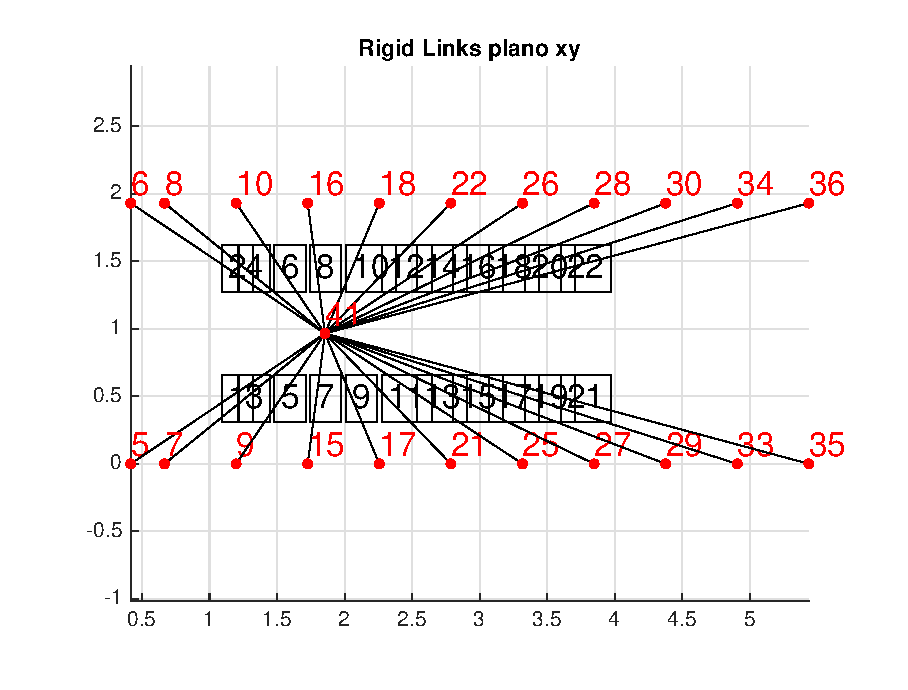
\includegraphics[width=\linewidth]{fig/modelRLxy.eps}
		\caption{Rigid links. Vista en plano $x\!y$.}
		\label{fig:modeloRLxy}
	\end{subfigure}
	\begin{subfigure}{0.49\textwidth}
		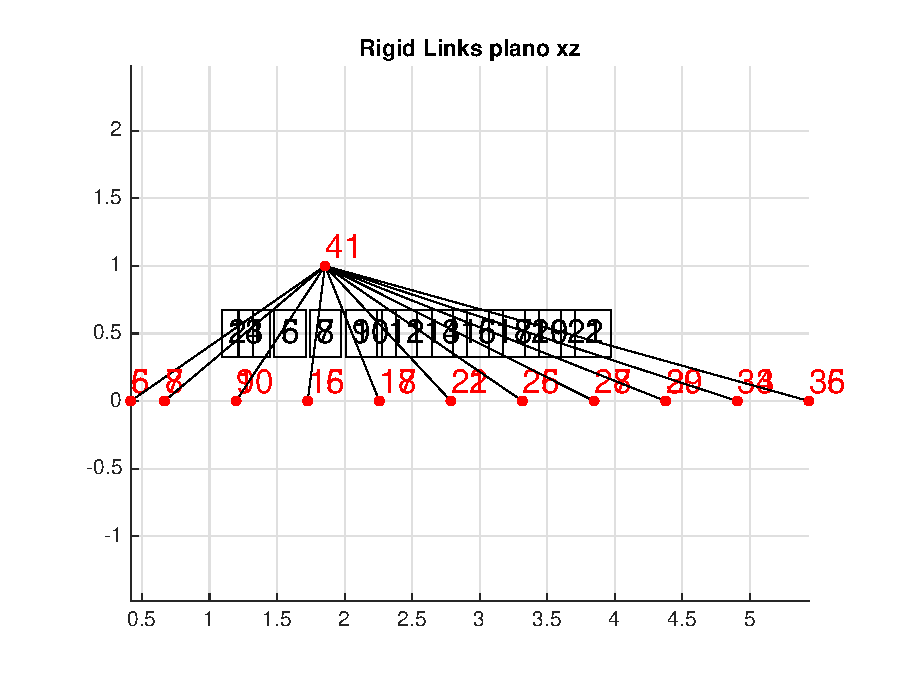
\includegraphics[width=\linewidth]{fig/modelRLxz.eps}
		\caption{Rigid links. Vista en plano $x\!z$.}
		\label{fig:modeloRLxz}
	\end{subfigure}
\end{figure}

\begin{figure}[htb!]
	\centering
	\includegraphics[width=0.8\textwidth]{fig/modelbasamento.eps}
	\caption{Modelo Basamento. Vista en plano $x\!y$.Tome en cuenta que los nodos numerados no necesariamente tienen que coincidir con figura de rigid links.}
	\label{fig:modelobasamento}
\end{figure}

\subsection*{Selección de parámetros}
Para un primer análisis se fijaron las distancias entre los bulones de tal forma como para que tengan el mismo espacio entre ellos. Se resuelve el problema para solicitaciones cuasiestáticas (peso de motor) para obtener la optima posición de los soportes en $y$.


\begin{table}[htb!]
	\centering
	\begin{tabular}{lllll}
		& 1 & 2 & 3 & 4 \\ \hline
		Uniones Abulonadas& 0,097 \si{\meter}  & 1,897 \si{ \meter} & 3,697 \si{ \meter} & 5,567 \si{ \meter} \\
		Soportes en $y$& 0,700 \si{\meter}  &1,700\si{\meter}   & 2,500 \si{\meter}  &  \\
	\end{tabular}
\caption{Posición en $x$ de los nodos correspondientes a los bulones que unen doble fondo con basamento y las vigas estructurales en $y$.}
\end{table}

Para dimensionar las vigas del basamento se comenzó resolviendo el sistema cuasiestático donde la única carga es el peso del motor. Esto dará un rango de dimensiones inicial para trabajar el problema dinámicamente y además se aprovechara posicionar los soportes en $y$ de tal forma que reduzcan las tensiones en régimen cuasiestático. 

Se considera que el amortiguamiento del sistema está controlado por la resina en los bulones para el análisis dinámico. Se decidió modelar esto como un amortiguamiento global de $\dampfact = 0,1$ en un análisis con amortiguamiento modal. La excitación $\omega_{\mathrm{exc}}$ es de 600 rpm y se calcula la amplitud de excitación según un desplazamiento de $10$mm sobre la masa puntual en la dirección $z$.

Por último se va efectuar un análisis con amortiguamiento proporcional usando la primer frecuencia natural del sistema como $\omega_1$ y $\omega_2 = 1,15 \omega_{\mathrm{exc}}$. Se amortiguan estos modos con $\dampfact_{1}=0,073$ y $\dampfact_2=0,2$, respectivamente. El desarrollo de esta formulación queda detallada en la parte B de este informe.

\section{Resultados del dimensionamiento}
En base al dimensionamiento estático se elige entonces una viga rectangular $h=70\si{\milli \meter}$ y $b=45\si{\milli \meter}$. Dada viga es sometida a una tensión máxima de $45$MPa bajo el peso del motor. Un cambio pequeño de sección (reducción de $5$mm de $b$) ocasionaba un fuerte incremento en las tensiones, casi duplicando la tensión por momentos flexores.

Un barrido en frecuencia (figura \ref{fig:sinesweepA}) revela la posibilidad que se trabaja cerca a una frecuencia natural, aunque no es del todo seguro ya que \textbf{pequeños} cambios en el amortiguamiento (aumentando o disminuyendo $\zeta_1$ y $\zeta_2$) disminuyen el pico obtenido. Cabe destacar que la amplitud para esta frecuencia natural es menor a la que se tiene en régimen cuasiestático. En cualquier caso, la zona de trabajo queda afuera del pico por un margen considerable.




\begin{figure}[htb!]
	\centering
	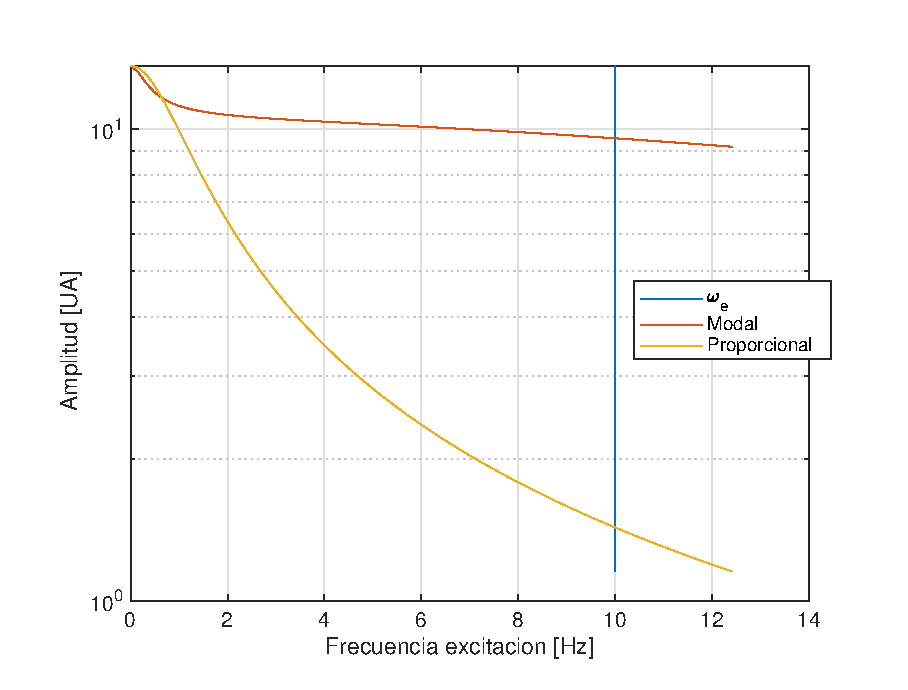
\includegraphics[width=0.6\textwidth]{fig/sinesweep.eps}
	\caption{Barrido de frecuencias en el rango de trabajo con vigas $h=70$mm y $b=45$mm. $\omega_{\mathrm{exc}}$ es la frecuencia de trabajo del motor. Note que las unidades son arbitrarias para ambas amplitudes.}
	\label{fig:sinesweepA}
\end{figure}



\subsection*{Optimización teórica}
Para la optimización teórica se resolvió el sistema integrando la ecuación \ref{eq:FuerzasDinamicas} mediante el método de Runge--Kutta para obtener la respuesta ante la excitación. Se varió la sección y luego $\alpha$ y $\beta$ del amortiguamiento (proporcional) \cite{cook2007concepts} para reducir las cargas transmitidas y desplazamientos. La mejor respuesta ante tensiones fue dada con $\alpha=0,002$ y $\beta = 0,00002$ y una sección de $h=0,070$m y $b=0,045$m. Cabe destacar que los valores obtenidos de la dimensión estática resultaron satisfactorios para el análisis de optimización teórica. Las tensiones por flexión de las vigas sobre los bulones se vé en las figuras \ref{fig:tensionBulon} y \ref{fig:tensionBulonRigid} \textbf{calculada en el tiempo}. Tener en cuenta que la máxima tensión fue hallada sobre un bulón conectado a un rigid beam (ver subtitulo de figuras mencionadas). Se calculo ante la flexión porque el modo de deformación es principalmente por flexión (\ref{fig:NoLineal}).

\section{Conclusión}
Podemos ver en la figura \ref{fig:tensionBulonRigid} que la tensión ($\approx 380$MPa) se acerca a los límites superiores de un acero que trabaja a fatiga, sin embargo, este nodo se encuentra conectado a un rigid beam que transmite la carga de la excitación. Esto no es fiel a la realidad, pues el motor iría apoyado y transmitiría los esfuerzos sobre una superficie. A diferencia las tensiones máximas sobre los bulones que no van conectados a rigid beams no superan los 100MPa. 

Sobre el tema de amortiguamiento proporcional, el valor elegido para $\alpha$ amortigua los modos bajos, su elección contribuyó a disminuir los esfuerzos transmitido, sin embargo la forma de calcular la matriz $\Mme{C}$ es una aproximación. Lograr el amortiguamiento calculado puede no ser posible.

En conclusión, se puede apreciar como el comportamiento de un sistema con masa (el motor) sometido a una excitación  puede verse afectado por variables como la rigidez de su apoyo y la energía puede disipar este apoyo.


\begin{figure}[htb!]
	\centering
	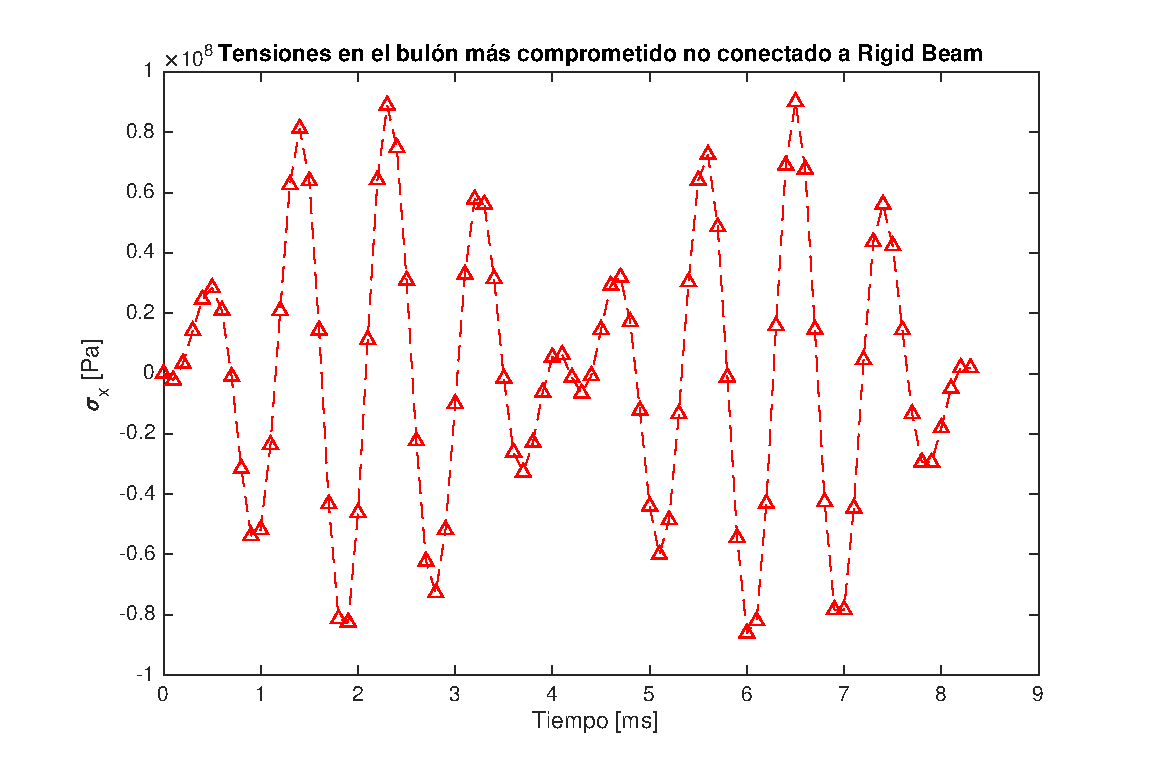
\includegraphics[width=.8\textwidth]{fig/tensionBulon.eps}
	
	\caption{Tensiones por flexión en el bulón más solicitado \textbf{no} conectado a rigid beam.}
	\label{fig:tensionBulon}
\end{figure}

\begin{figure}[htb!]
	\centering
	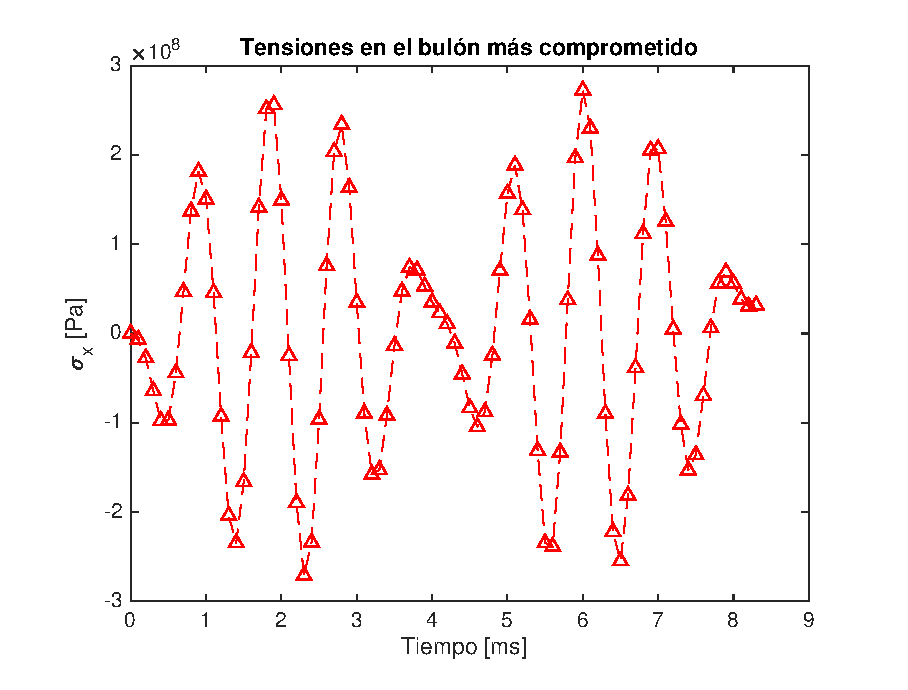
\includegraphics[width=.7\textwidth]{fig/tensionBulonRigid.eps}
	\caption{Tensiones máximas obtenidas en el bulón más solicitado}
	\label{fig:tensionBulonRigid}
\end{figure}

\begin{figure}[htb!]
	\centering
	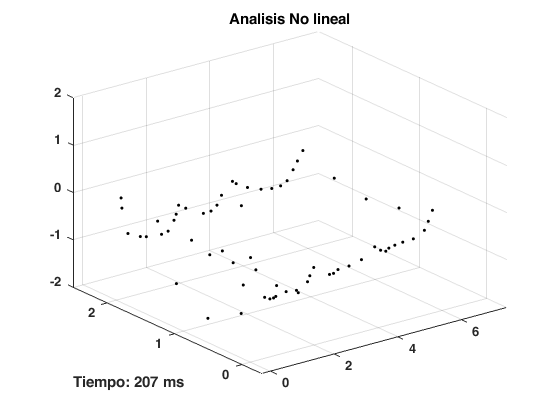
\includegraphics[width=.7\textwidth]{fig/analisisNoLineal.png}
	\caption{Respuesta del basamento para la excitación en un instante de tiempo. Desplazamientos magnificados $\times 50$. Note que el modo de deformación es principalmente en flexión.}
	\label{fig:NoLineal}
\end{figure}


\bibliography{labibliografia} % Indica archivo
\bibliographystyle{plainnat} 

\end{document}